\presec
\section{Evaluation of \taskpara{} \; of \sketchname} \postsec
\label{eva_para}

\begin{figure*}[!ht]
	\centering
	%
	\subfigure[Synthetic dataset]{
				\begin{minipage}[t]{0.26\textwidth}{
						\prefig\begin{center}
							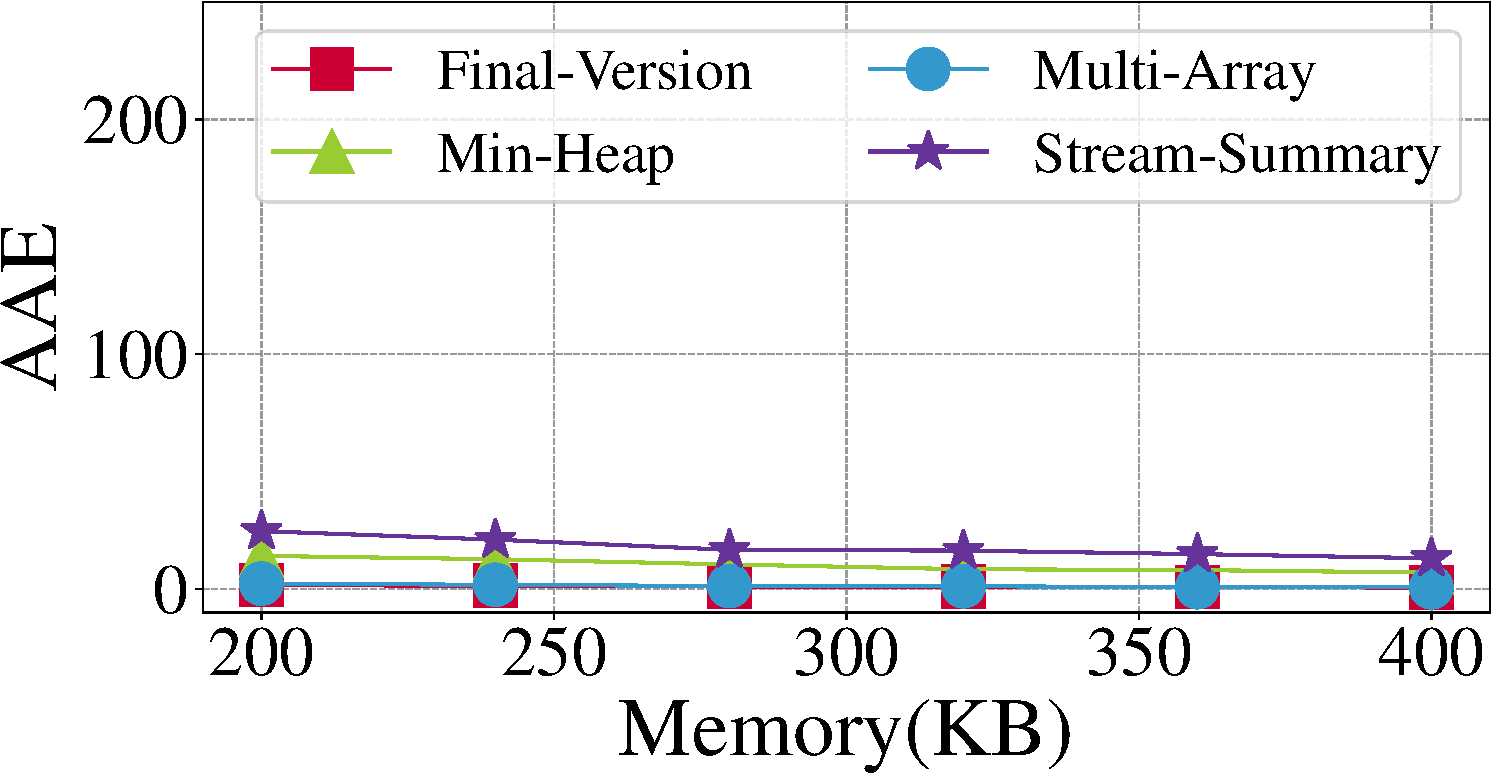
\includegraphics[width=0.95\textwidth, ]{Figures/str_syn_aae-cropped.pdf}\end{center}}
					\postfig \adjustfigs\prefigcaption
					\label{str_aae_syn}\postfigcaption
					%					
				\end{minipage}}
				%
	\subfigure[IP trace]{
		\begin{minipage}[t]{0.23\textwidth}{
				\prefig
				\begin{center}
					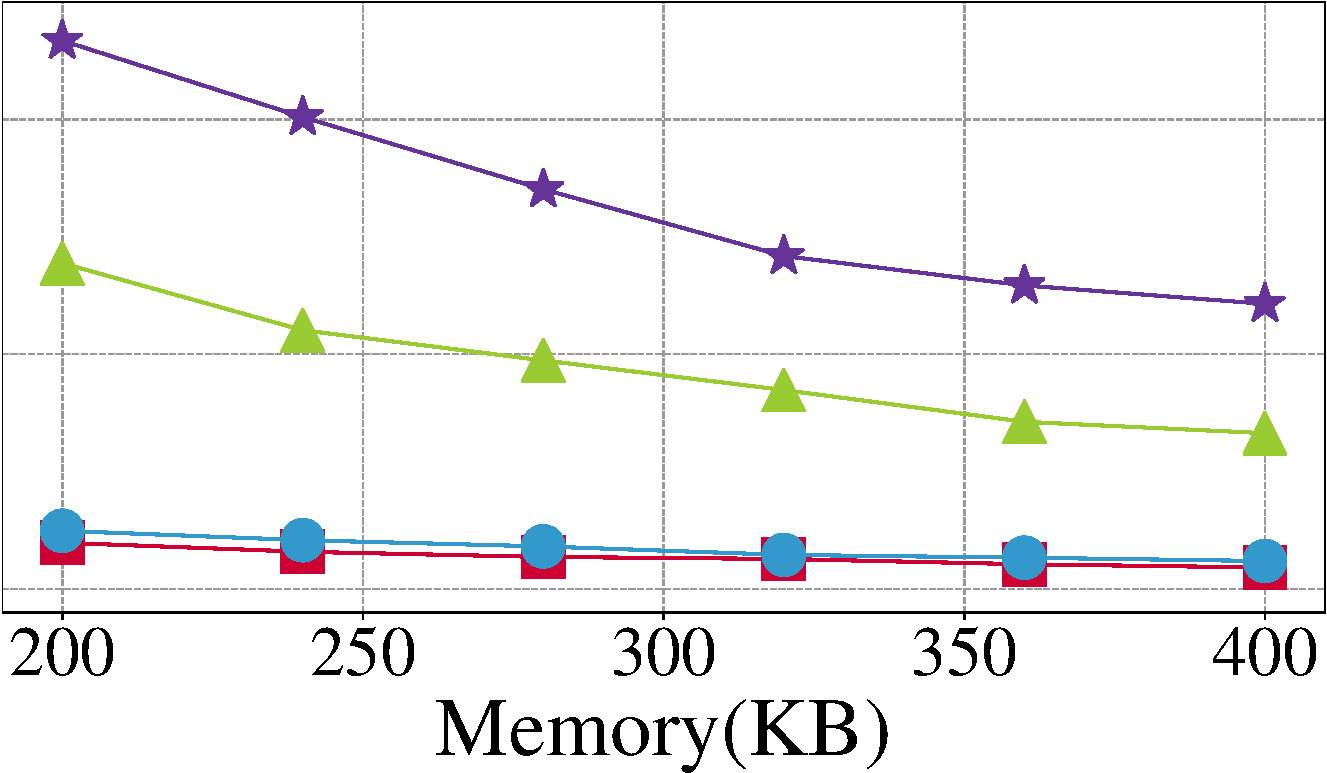
\includegraphics[width=0.95\textwidth, ]{Figures/str_ip_aae-cropped.pdf}
					\end{center}}
			\postfig\adjustfigs\prefigcaption
			\label{str_aae_ip}\postfigcaption
		\end{minipage}}
		%
		\subfigure[Web page]{
			\begin{minipage}[t]{0.23\textwidth}{
					\prefig
					\begin{center}		
						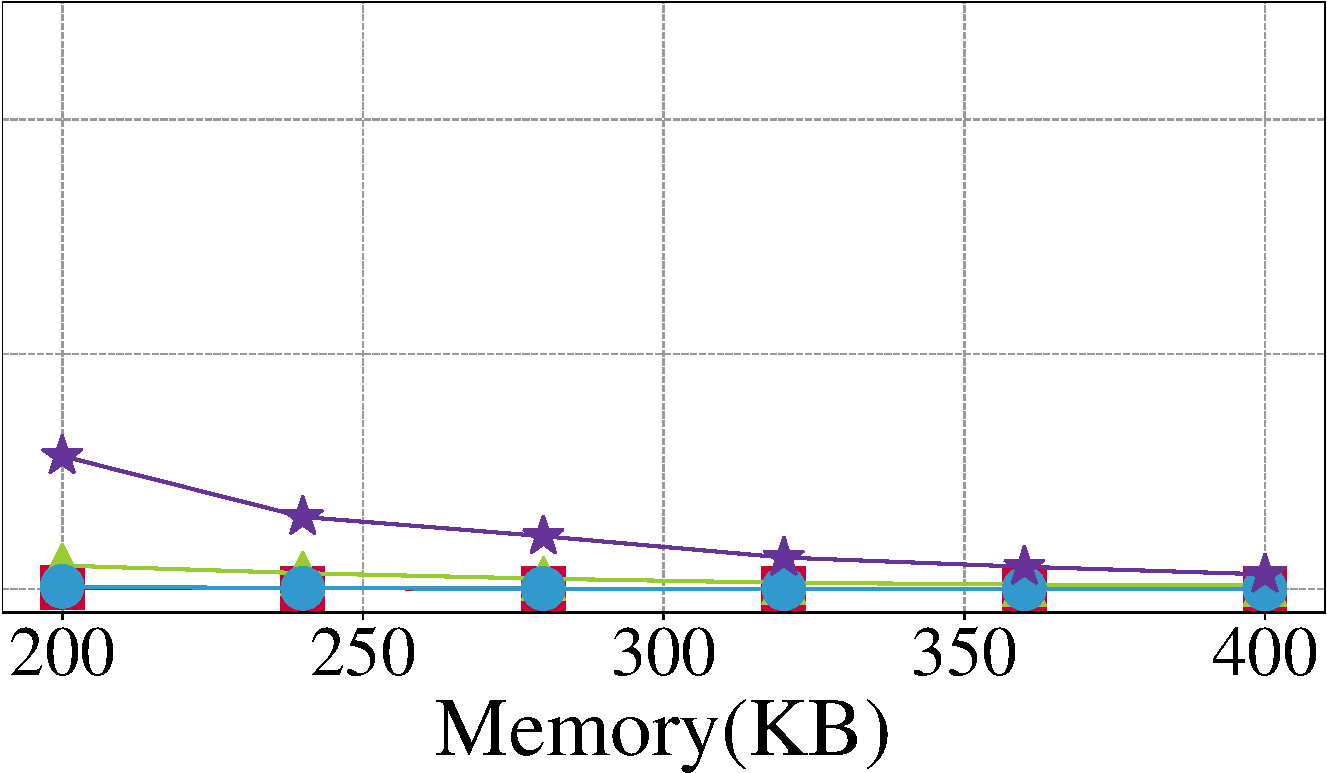
\includegraphics[width=0.95\textwidth]{Figures/str_web_aae-cropped.pdf}\end{center}}
				\postfig \adjustfigs\prefigcaption
				\label{str_aae_web}\postfigcaption
			\end{minipage}}
			%
					%
		\subfigure[Network dataset]{
			\begin{minipage}[t]{0.23\textwidth}{
					\prefig
					\begin{center}		
						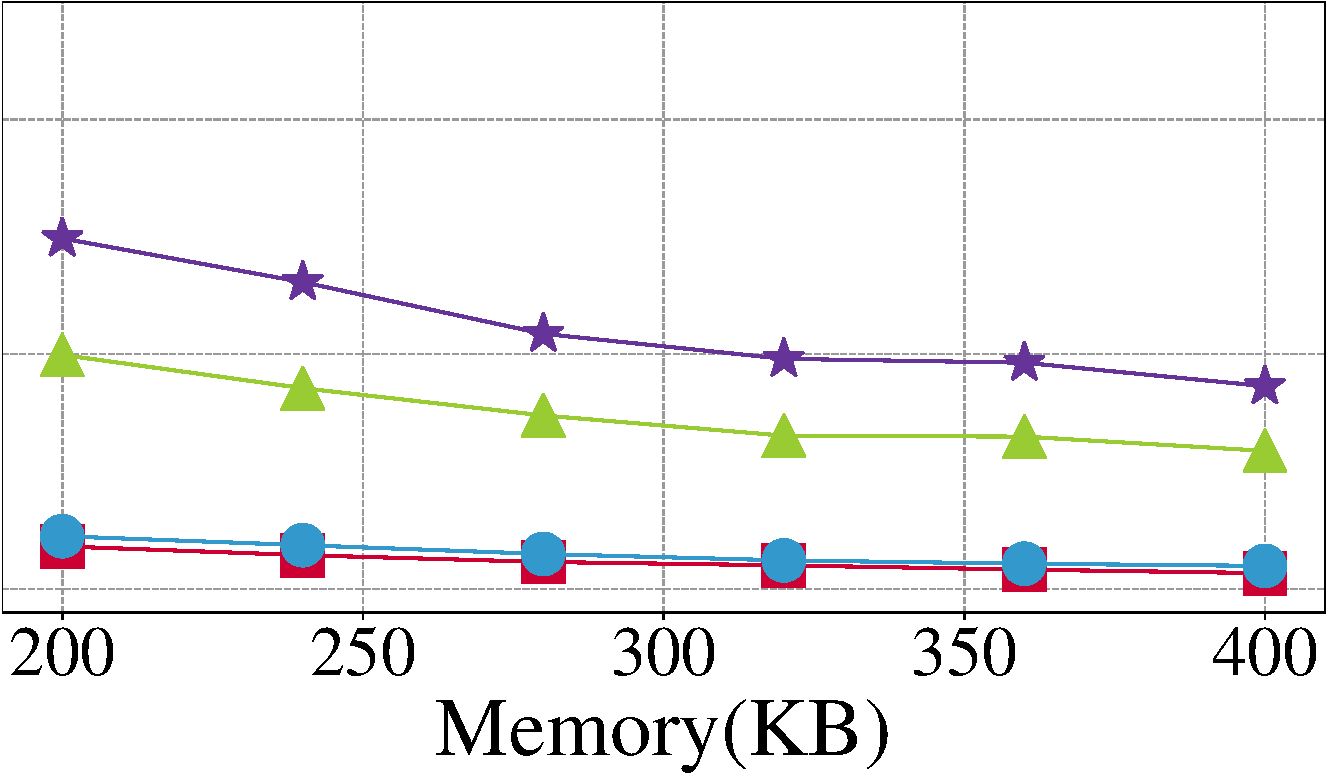
\includegraphics[width=0.95\textwidth]{Figures/str_net_aae-cropped.pdf}\end{center}}
				\postfig \adjustfigs\prefigcaption
				\label{str_aae_net}\postfigcaption
			\end{minipage}}
			%
				\caption{AAE on \taskpara.}
				\label{str_aae}
			\end{figure*}

\begin{figure*}[!ht]
	\centering
	%1.065
	\subfigure[Synthetic dataset]{
				\begin{minipage}[t]{0.263\textwidth}{
						\prefig\begin{center}
							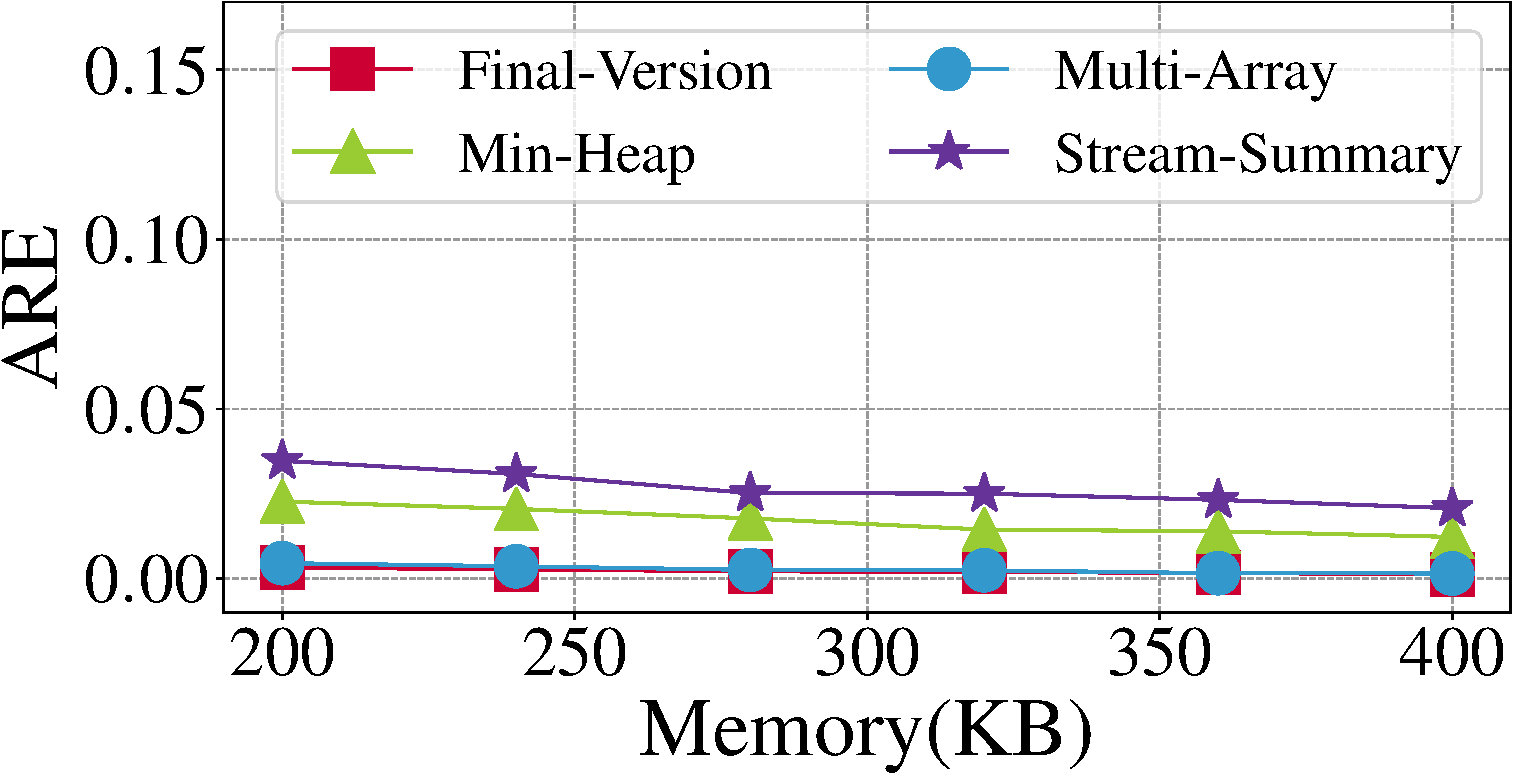
\includegraphics[width=0.95\textwidth, ]{Figures/str_syn_are-cropped.pdf}\end{center}}
					\postfig \adjustfigs\prefigcaption
					\label{str_are_syn}\postfigcaption
					%					
				\end{minipage}}
				%
	\subfigure[IP trace]{
		\begin{minipage}[t]{0.23\textwidth}{
				\prefig
				\begin{center}
					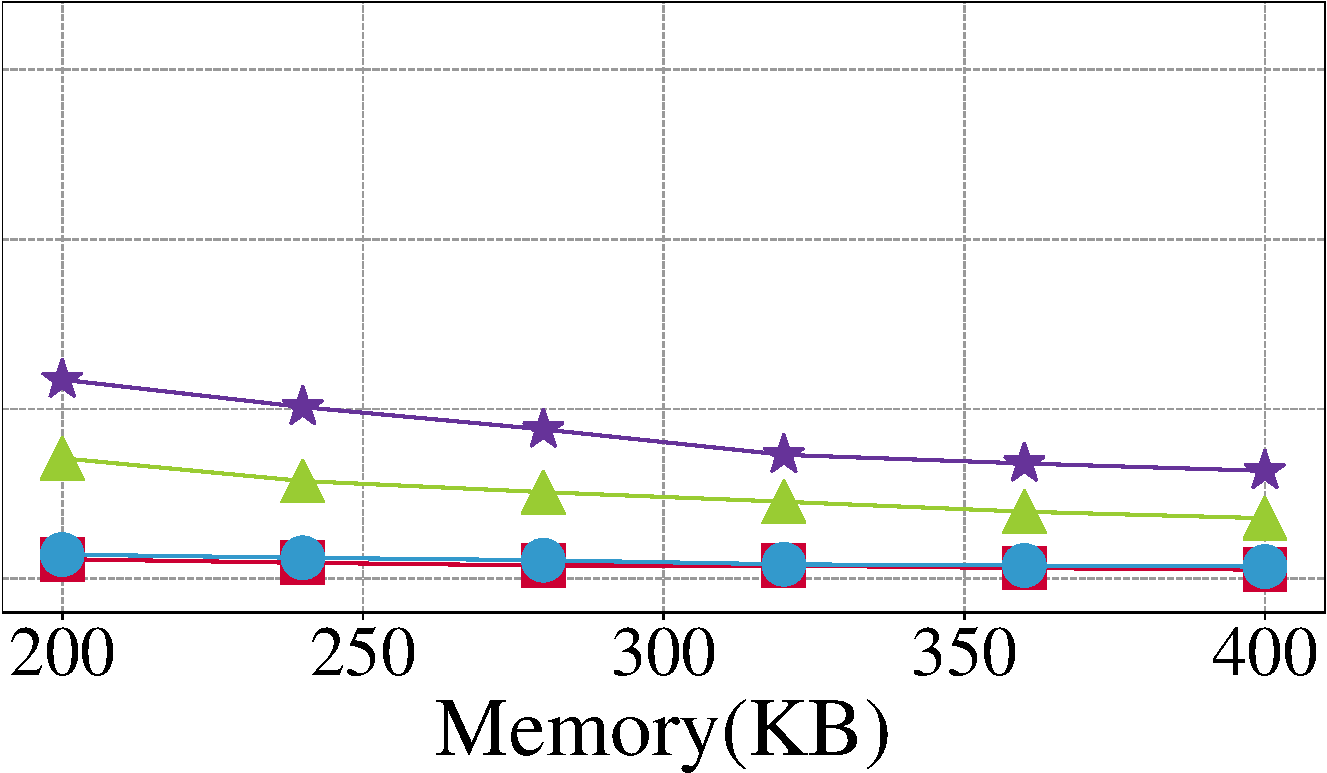
\includegraphics[width=0.95\textwidth, ]{Figures/str_ip_are-cropped.pdf}
					\end{center}}
			\postfig\adjustfigs\prefigcaption
			\label{str_are_ip}\postfigcaption
		\end{minipage}}
		%
		\subfigure[Web page]{
			\begin{minipage}[t]{0.23\textwidth}{
					\prefig
					\begin{center}		
						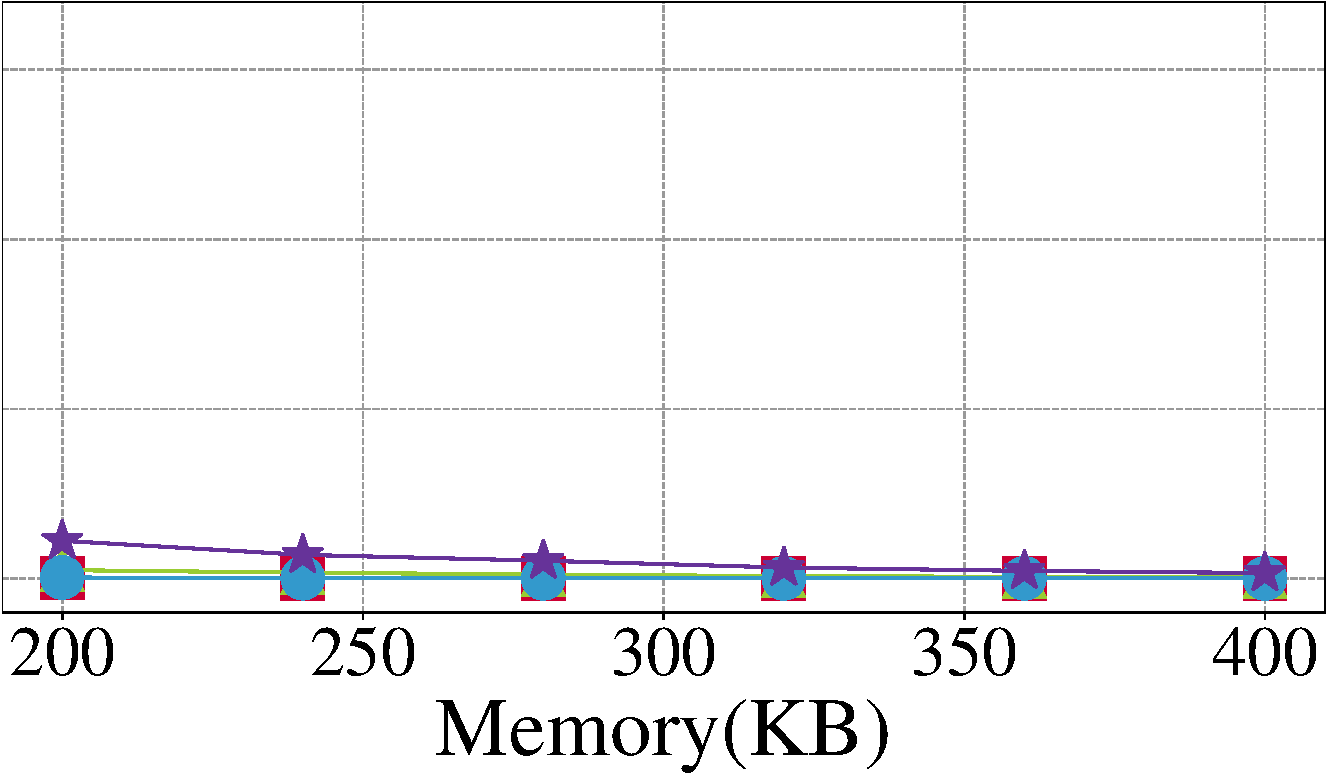
\includegraphics[width=0.95\textwidth, ]{Figures/str_web_are-cropped.pdf}\end{center}}
				\postfig \adjustfigs\prefigcaption
				\label{str_are_web}\postfigcaption
			\end{minipage}}
			%
					%
		\subfigure[Network dataset]{
			\begin{minipage}[t]{0.23\textwidth}{
					\prefig
					\begin{center}		
						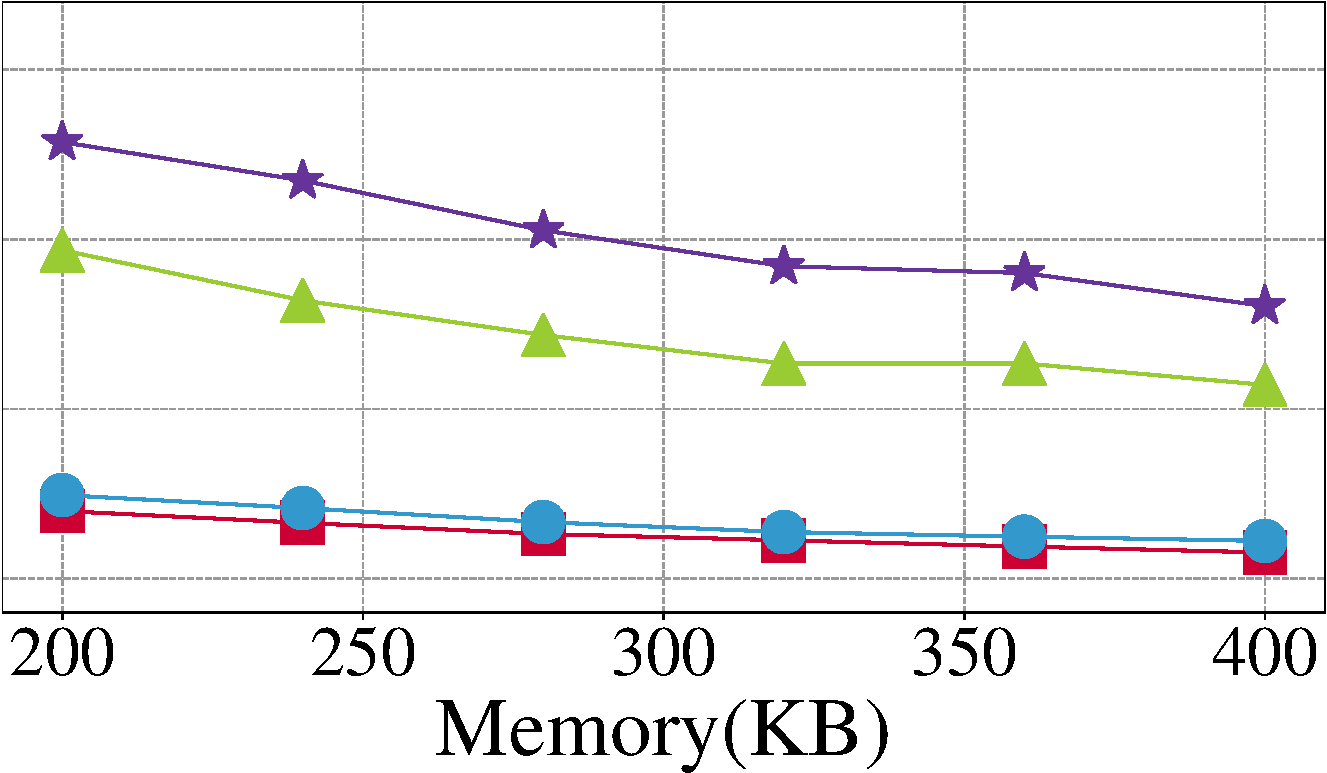
\includegraphics[width=0.95\textwidth, ]{Figures/str_net_are-cropped.pdf}\end{center}}
				\postfig \adjustfigs\prefigcaption
				\label{str_are_net}\postfigcaption
			\end{minipage}}
			%
			
				\caption{ARE on \taskpara.}
				\label{str_are}
			\end{figure*}			

\begin{figure*}[!ht]
	\centering
	%1.1087
	\subfigure[Synthetic dataset]{
				\begin{minipage}[t]{0.256\textwidth}{
						\prefig\begin{center}
							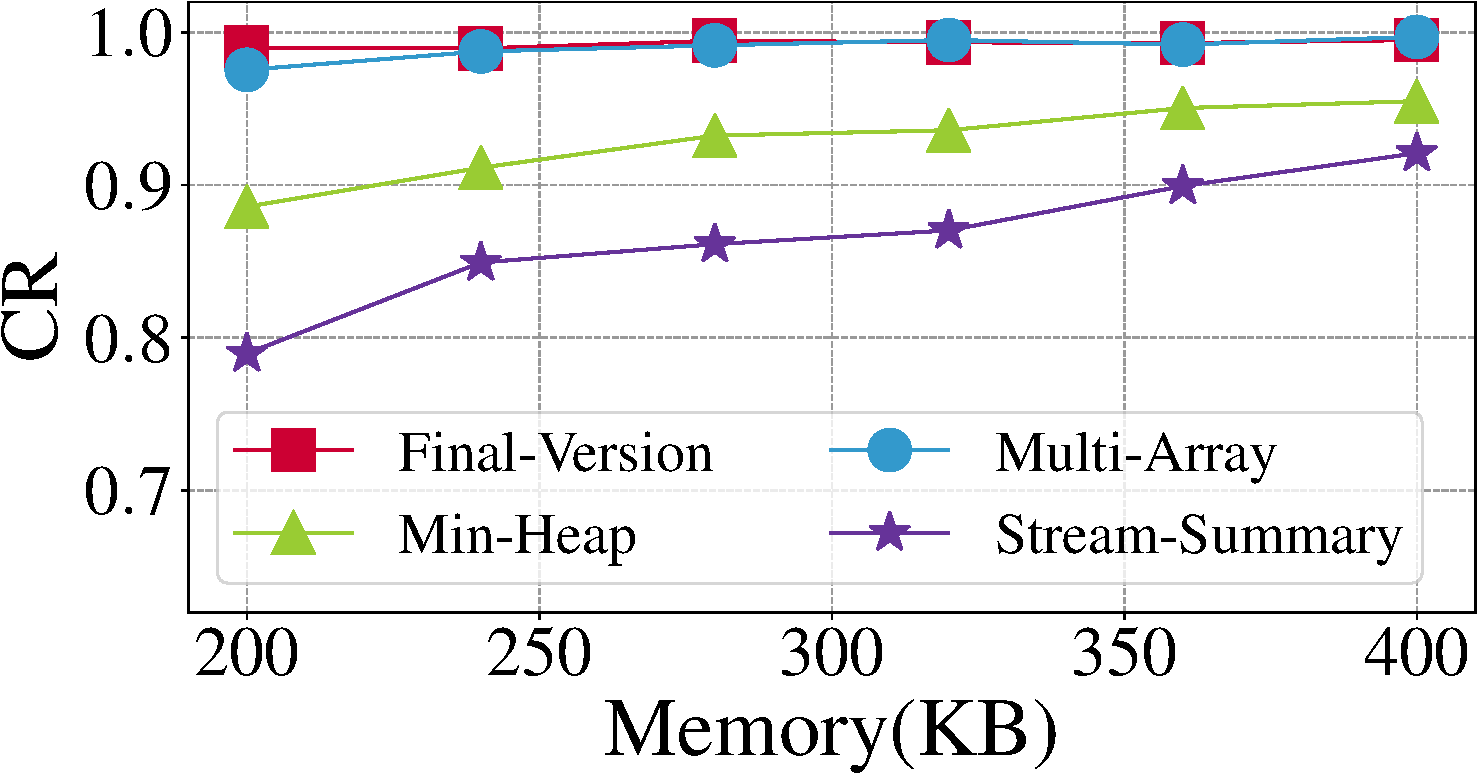
\includegraphics[width=0.95\textwidth, ]{Figures/str_syn_cr-cropped.pdf}\end{center}}
					\postfig \adjustfigs\prefigcaption
					\label{str_cr_syn}\postfigcaption
					%					
				\end{minipage}}
				%
	\subfigure[IP trace]{
		\begin{minipage}[t]{0.23\textwidth}{
				\prefig
				\begin{center}
					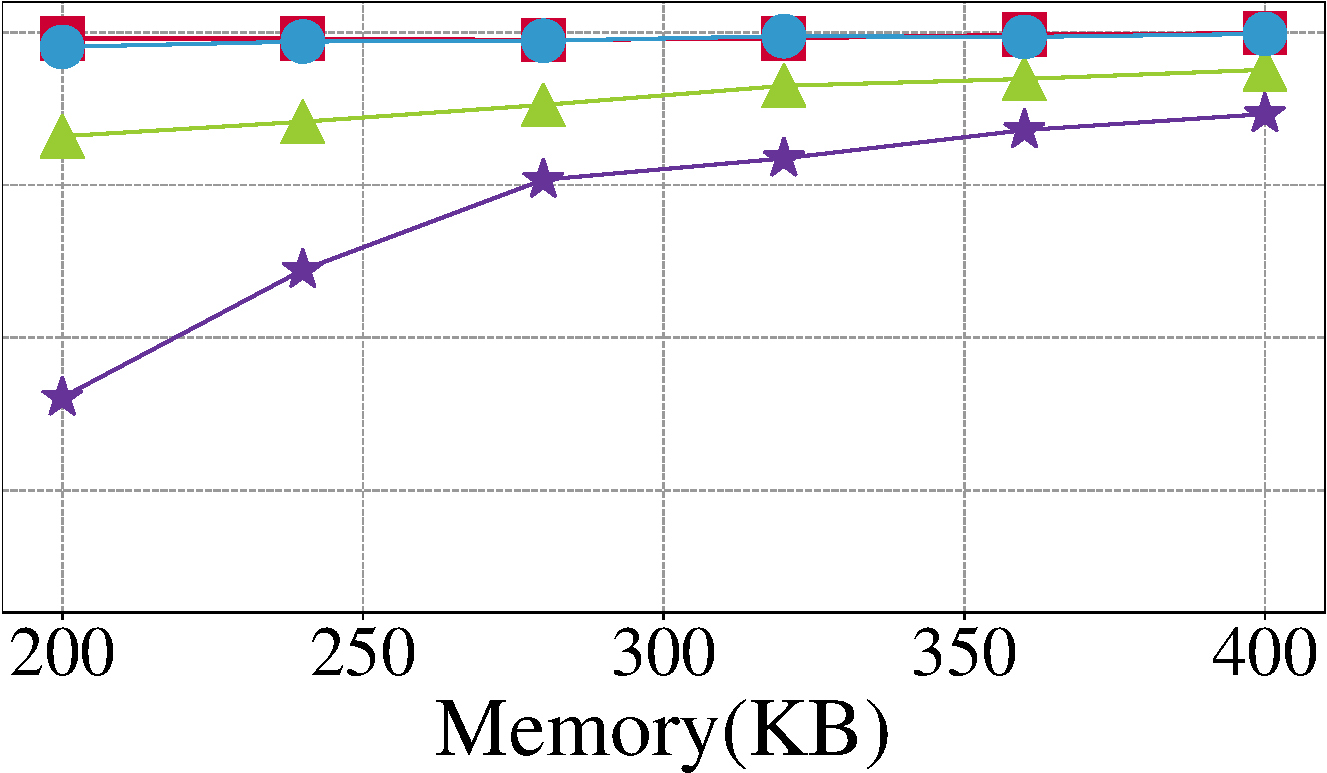
\includegraphics[width=0.95\textwidth, ]{Figures/str_ip_cr-cropped.pdf}
					\end{center}}
			\postfig\adjustfigs\prefigcaption
			\label{str_cr_ip}\postfigcaption
		\end{minipage}}
		%
		\subfigure[Web page]{
			\begin{minipage}[t]{0.23\textwidth}{
					\prefig
					\begin{center}		
						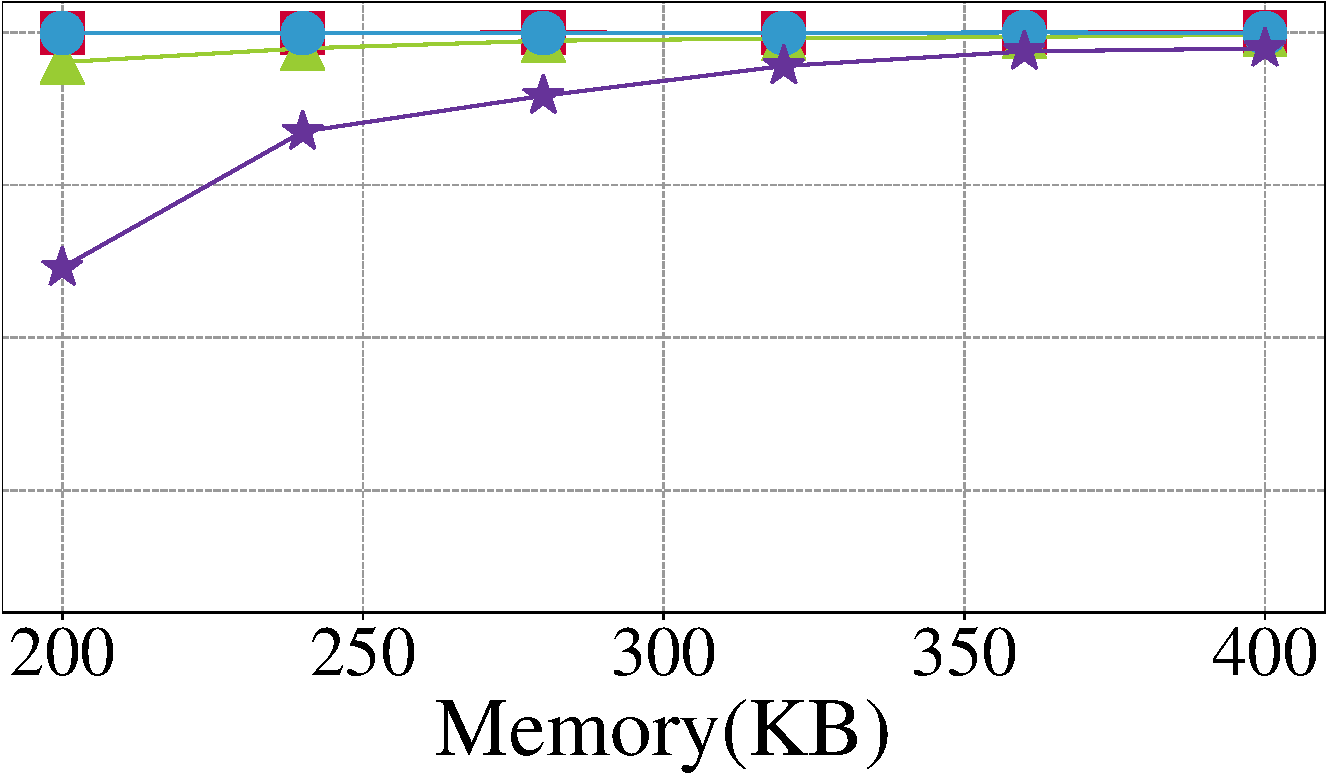
\includegraphics[width=0.95\textwidth, ]{Figures/str_web_cr-cropped.pdf}\end{center}}
				\postfig \adjustfigs\prefigcaption
				\label{str_cr_web}\postfigcaption
			\end{minipage}}
			%
					%
		\subfigure[Network dataset]{
			\begin{minipage}[t]{0.23\textwidth}{
					\prefig
					\begin{center}		
						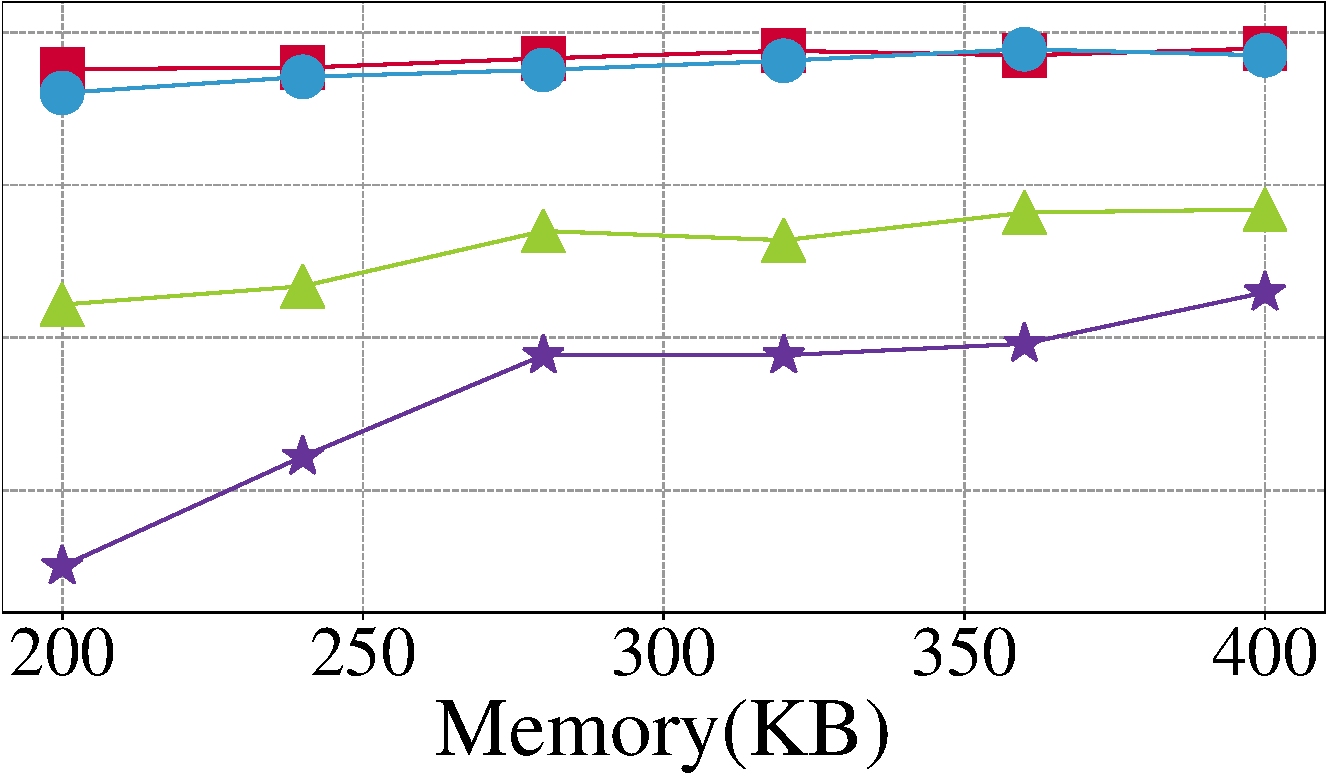
\includegraphics[width=0.95\textwidth, ]{Figures/str_net_cr-cropped.pdf}\end{center}}
				\postfig \adjustfigs\prefigcaption
				\label{str_cr_net}\postfigcaption
			\end{minipage}}
			%

			
				\caption{CR on \taskpara.}
				\label{str_cr}
				
			\end{figure*}
			
\noindent\textbf{Parameter Setting:}
%We compare three frameworks: \sketchname, \EHname and \Splittername. For each frameworks, we using CM Sketch, CM-CU Sketch and Count Sketch approaches.
%
%We compare 5 approaches: CM \sketchname, CM-CU \sketchname, Count \sketchname, \EHname {} and \Splittername.
%

We compare 4 versions of \sketchname, \secmin, \secss, \secarr, and the final version. These different versions are introduced in Section~\ref{sec:optimization}.
Let $c$ be the number of arrays. In the version using Multi-Array, we set $c=4$.
Let $d$ be the number of cells in each bucket. For the final version of \sketchname, we set $d=8$.
In this experiment, we compare AAE, ARE, PR, CR, and insertion speed among the 4 versions.
We focus on finding the frequent items to ignore the errors brought by the Bloom filter.   

			
\noindent\textbf{AAE (Figure~\ref{str_aae_syn}-\ref{str_aae_net}):}
We find that, on three real-world datasets and one synthetic dataset, the AAE of the final version of \sketchname{} is around 10 times, 20 times, and 1.3 times lower than \secmin, \secss, and \secarr, respectively. 
			
			
\noindent\textbf{ARE (Figure~\ref{str_are_syn}-\ref{str_are_net}):}
We find that, on three real-world datasets and one synthetic dataset, the ARE of the final version of \sketchname{} is around 9 times, 14 times, and 1.3 times lower than \secmin, \secss, and \secarr, respectively. 
			
			
\noindent\textbf{CR (Figure~\ref{str_cr_syn}-\ref{str_cr_net}):}
We find that, on three real-world datasets and one synthetic dataset, the CR of the final version of \sketchname{} is around 1.1 times and 1.2 times lower than \secmin{} and \secss. Also, \secarr{} and the final version have nearly the same CR. 

\begin{figure*}[!ht]
	\centering
	%
	\subfigure[Synthetic dataset]{
				\begin{minipage}[t]{0.255\textwidth}{
						\prefig\begin{center}
							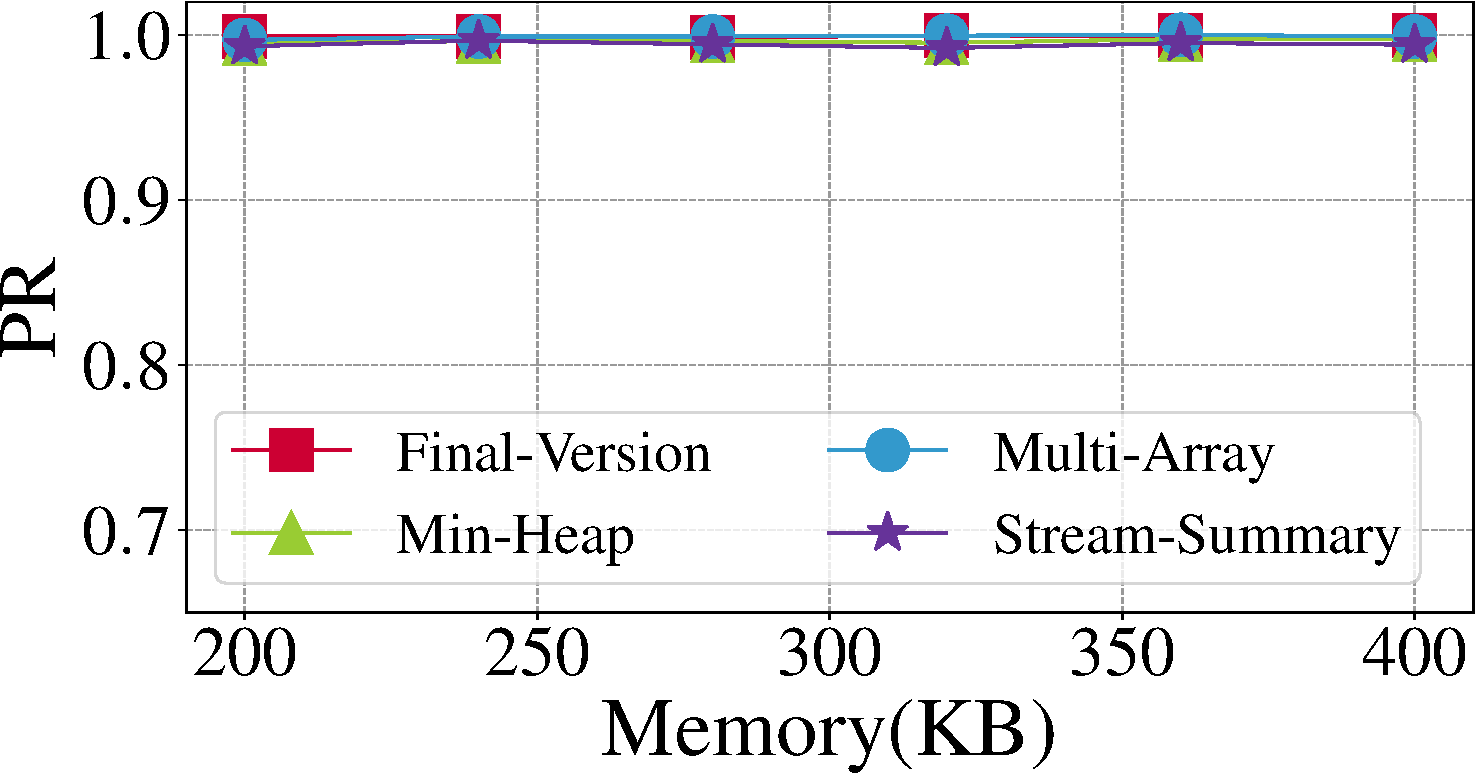
\includegraphics[width=0.95\textwidth, ]{Figures/str_syn_pr-cropped.pdf}\end{center}}
					\postfig \adjustfigs\prefigcaption
					\label{str_pr_syn}\postfigcaption
					%					
				\end{minipage}}
				%
	\subfigure[IP trace]{
		\begin{minipage}[t]{0.23\textwidth}{
				\prefig
				\begin{center}
					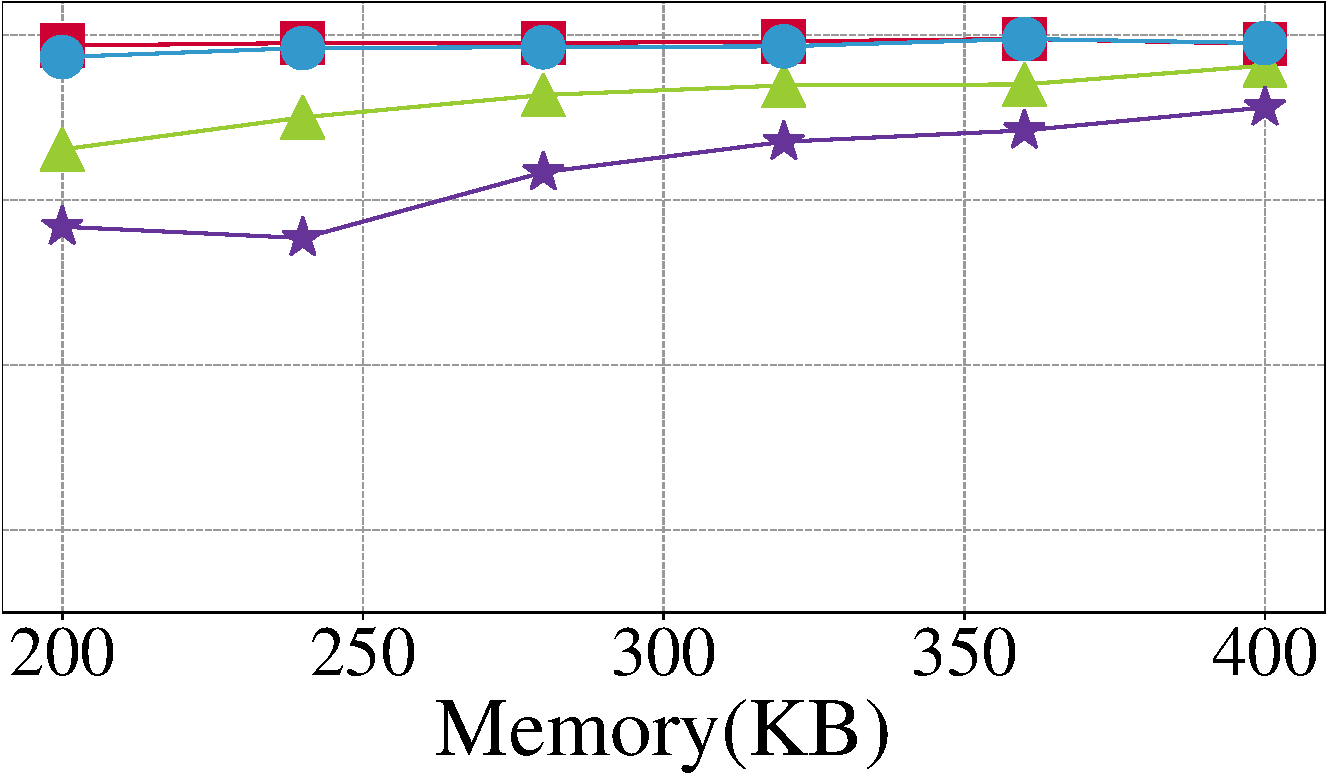
\includegraphics[width=0.95\textwidth, ]{Figures/str_ip_pr-cropped.pdf}
					\end{center}}
			\postfig\adjustfigs\prefigcaption
			\label{str_pr_ip}\postfigcaption
		\end{minipage}}
		%
		\subfigure[Web page]{
			\begin{minipage}[t]{0.23\textwidth}{
					\prefig
					\begin{center}		
						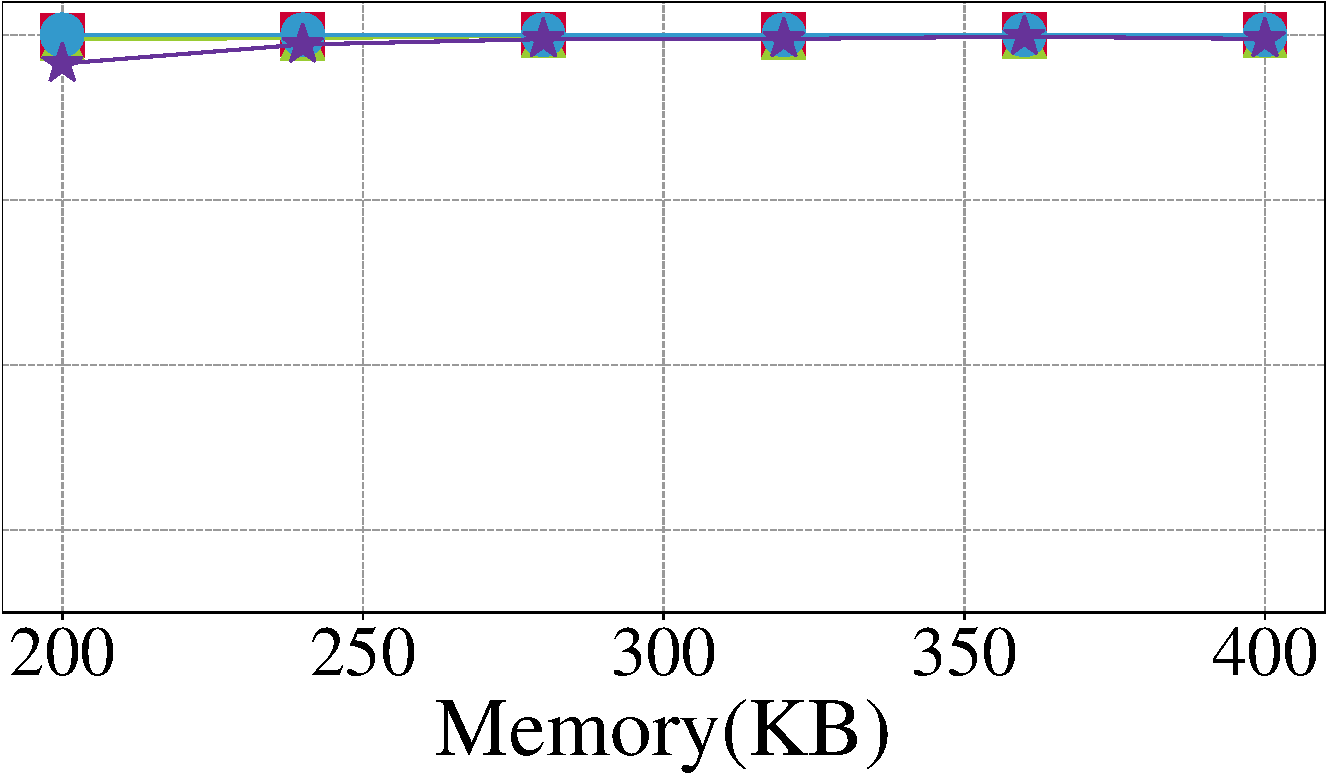
\includegraphics[width=0.95\textwidth, ]{Figures/str_web_pr-cropped.pdf}\end{center}}
				\postfig \adjustfigs\prefigcaption
				\label{str_pr_web}\postfigcaption
			\end{minipage}}
			%
					%
		\subfigure[Network dataset]{
			\begin{minipage}[t]{0.23\textwidth}{
					\prefig
					\begin{center}		
						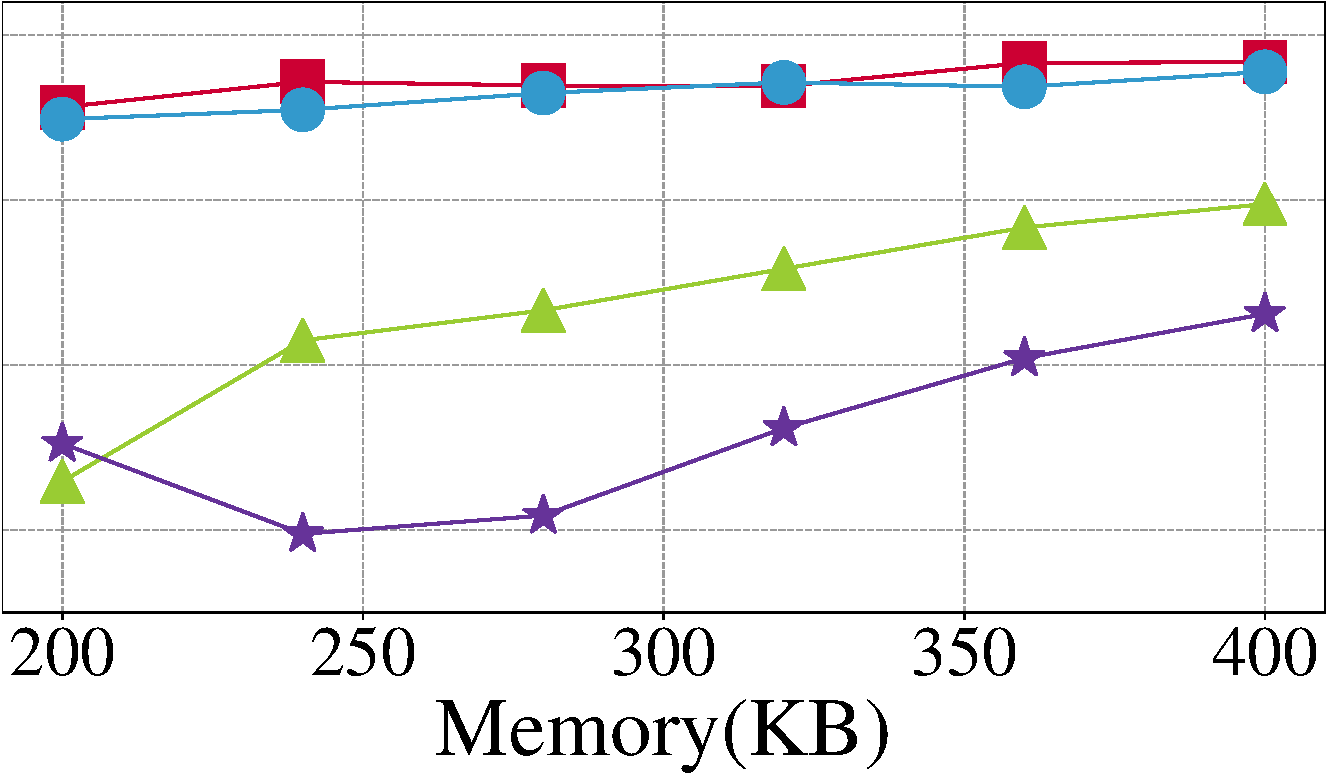
\includegraphics[width=0.95\textwidth, ]{Figures/str_net_pr-cropped.pdf}\end{center}}
				\postfig \adjustfigs\prefigcaption
				\label{str_pr_net}\postfigcaption
			\end{minipage}}
			%

			
				\caption{PR on \taskpara.}
				\label{str_pr}
				
			\end{figure*}
			
			
\noindent\textbf{PR (Figure~\ref{str_pr_syn}-\ref{str_pr_net}):}
We find that, on the Synthetic Dataset and the Web Page Dataset, these four version have nearly the same PR. On the IP Trace Dataset and the Network Dataset, \secss{} and \secmin{} perform worse than \secarr{} and the final version. 
			
\begin{figure*}[!ht]
	\centering
	%
	\subfigure[Synthetic dataset]{
				\begin{minipage}[t]{0.256\textwidth}{
						\prefig\begin{center}
							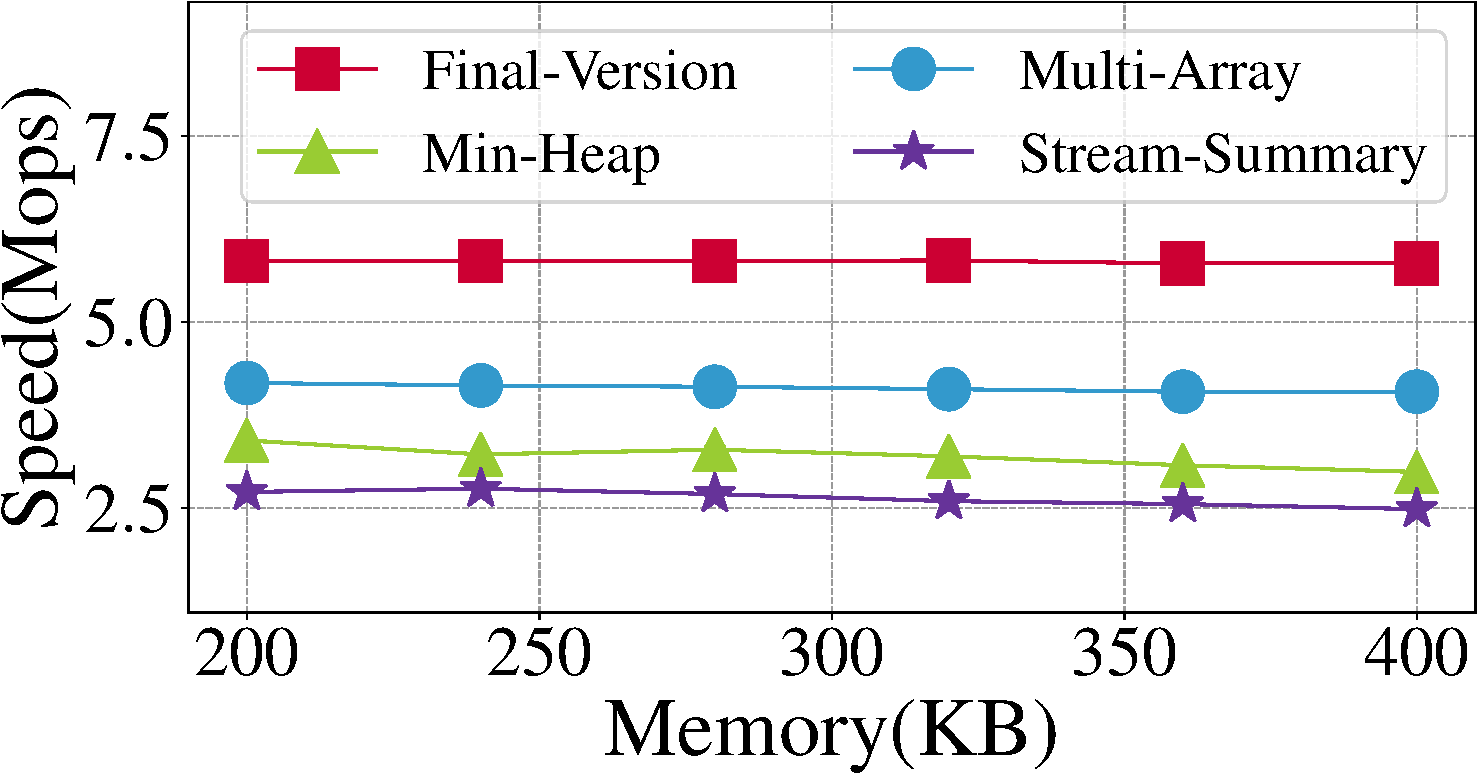
\includegraphics[width=0.95\textwidth, ]{Figures/str_syn_speed-cropped.pdf}\end{center}}
					\postfig \adjustfigs\prefigcaption
					\label{str_speed_syn}\postfigcaption
					%					
				\end{minipage}}
				%
	\subfigure[IP trace]{
		\begin{minipage}[t]{0.23\textwidth}{
				\prefig
				\begin{center}
					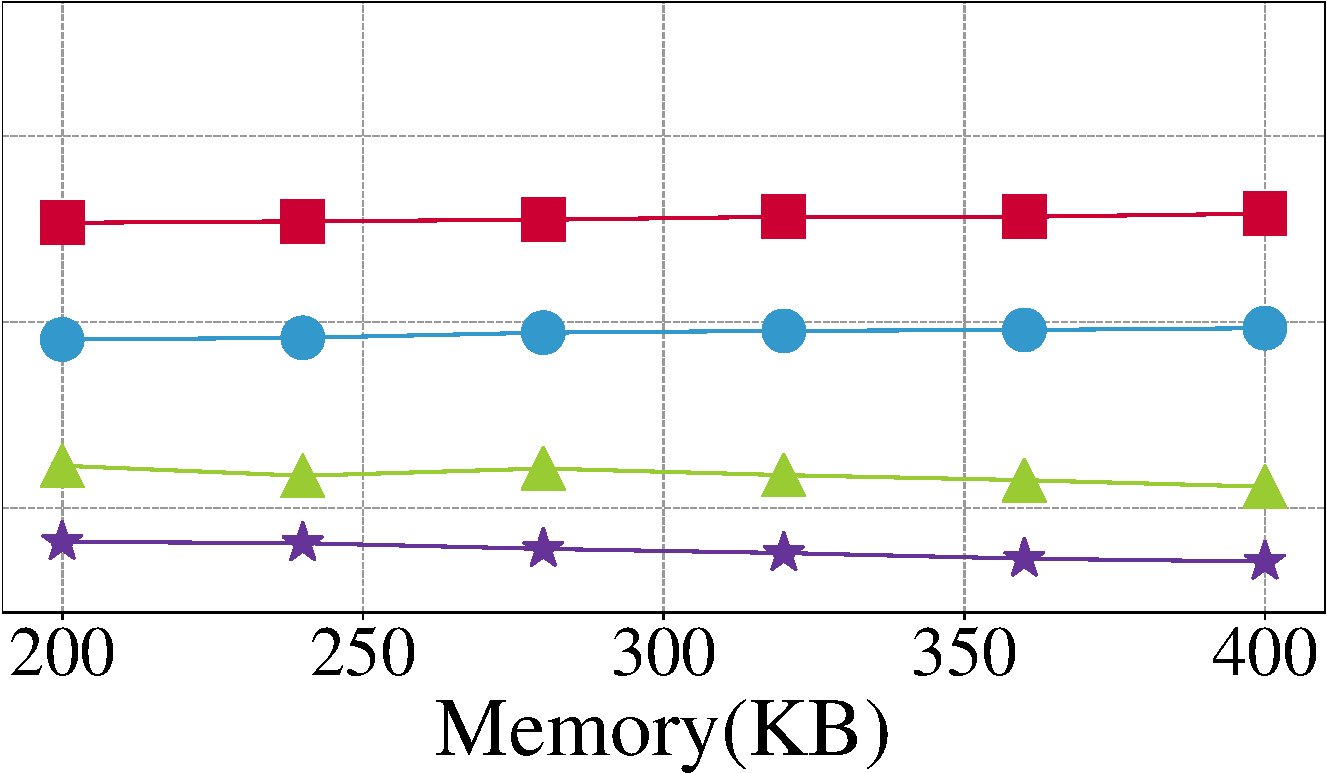
\includegraphics[width=0.95\textwidth, ]{Figures/str_ip_speed-cropped.pdf}
					\end{center}}
			\postfig\adjustfigs\prefigcaption
			\label{str_speed_ip}\postfigcaption
		\end{minipage}}
		%
		\subfigure[Web page]{
			\begin{minipage}[t]{0.23\textwidth}{
					\prefig
					\begin{center}		
						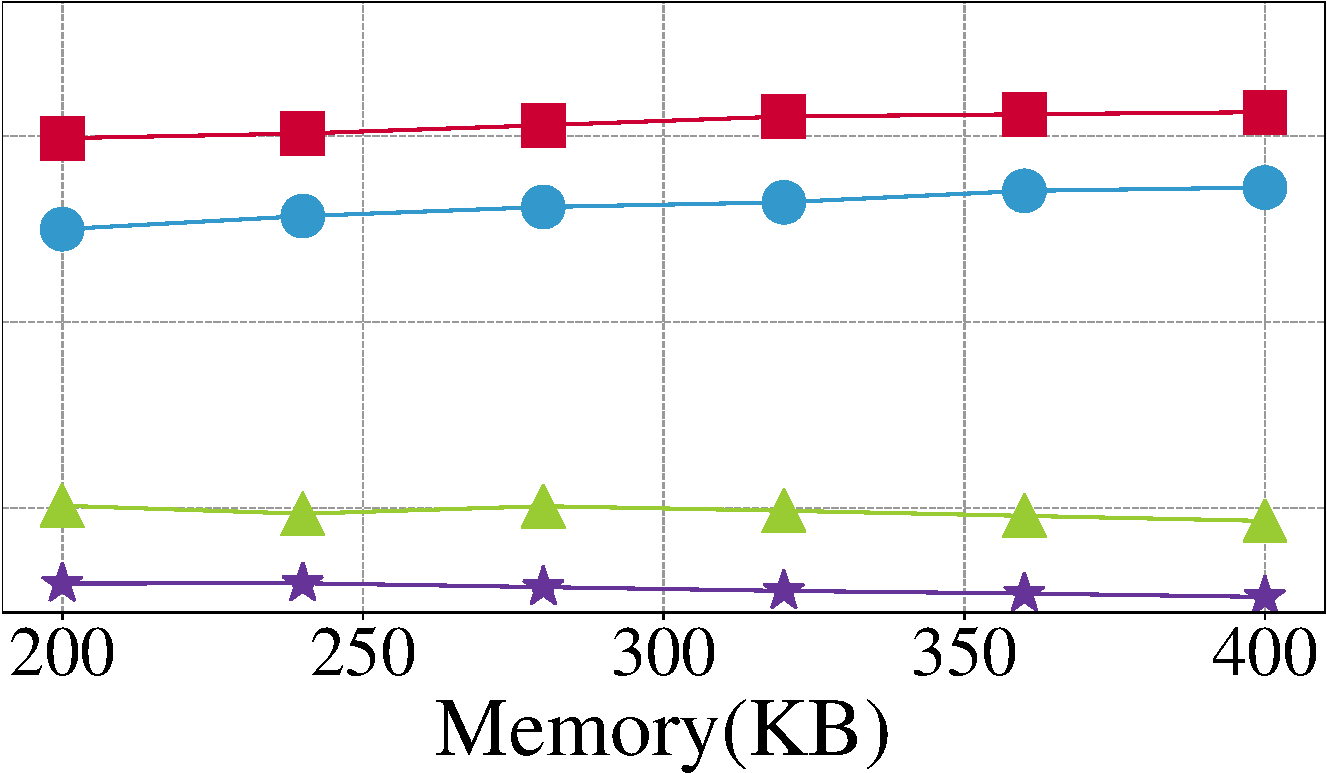
\includegraphics[width=0.95\textwidth, ]{Figures/str_web_speed-cropped.pdf}\end{center}}
				\postfig \adjustfigs\prefigcaption
				\label{str_speed_web}\postfigcaption
			\end{minipage}}
			%
					%
		\subfigure[Network dataset]{
			\begin{minipage}[t]{0.23\textwidth}{
					\prefig
					\begin{center}		
						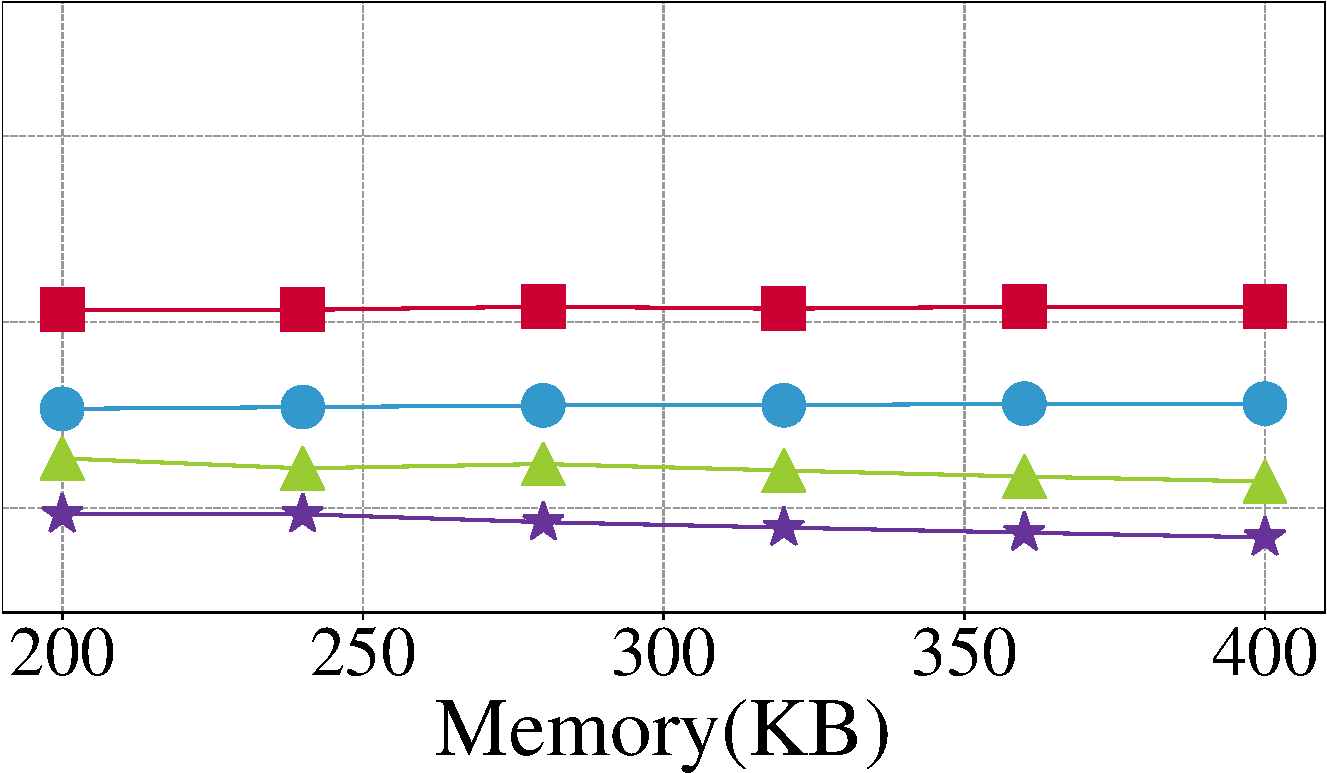
\includegraphics[width=0.95\textwidth, ]{Figures/str_net_speed-cropped.pdf}\end{center}}
				\postfig \adjustfigs\prefigcaption
				\label{str_speed_net}\postfigcaption
			\end{minipage}}
			%

			
				\caption{Speed on \taskpara.}
				\label{str_speed}
				
			\end{figure*}
			
			
\noindent\textbf{Speed (Figure~\ref{str_speed_syn}-\ref{str_speed_net}):}
We find that, on three real-world datasets and one synthetic dataset, the AAE of the final version of \sketchname{} is around 1.7 times, 2 times, and 1.4 times lower than \secmin, \secss, and \secarr, respectively. 

\noindent\textbf{Summary:}

1) The final version and \secarr{} achieve high accuracy with limited memory. Due to the memory cost of pointers and hash tables, \secss{} and \secmin{} cannot record as many items as \secarr{} and the final version. As a result, they will perform worse.

2) Though \secss{} achieves $O(1)$ time complexity, its insertion speed is the slowest among these 4 versions, because it needs to modify many pointers for each update. In contrast, though the time complexity of \secmin{} is $O(logk)$, its insertion speed is often faster than the one of \secss{}, because having too many items in the min-heap is rare. \secarr{} is slower than the final version because it needs to calculate more hash functions and access memory discontinuously.